% !TEX root = main.tex


\section{Implementierung}
\label{sec:implementierung}
%ToDo
%verweis auf github/gitlab link zum Projekt

\subsection{getUserMedia}
\label{subsec:getUserMedia}
Zu Beginn der Anwendung wird die Wiedergabequelle des Clients in Form eines MediaStream-Objektes abgerufen.
Die Umsetzung ist durch die \textit{getUserMedia-API()} sehr einfach und beschränkt sich auf wenige Zeilen-Code.

Hierbei wird der Benutzer aufgefordert dem Browser Zugriff auf eine Medienquelle zu gewähren, die einen MediaStream produziert der die angegebenen
Medientypen (Video und Audio) als Spuren (\textit{MediaStreamTrack}) enthält.
Anzumerken ist hierbei das die Methode \textit{getUserMedia()} asynchron ist.
Für die Nutzung der API außerhalb der lokalen Entwicklung (localhost) muss die Anwendung zudem über
HTTPS geladen werden (\textit{secure context}) \parencite{MozUserMediaSecurity}.

Nachdem dies erfolgt ist beginnt der Signaling-Prozess.

\subsection{Signaling}
\label{subsec:Signaling}
Für den Austausch der notwendigen Signaling-Nachrichten werden client- und serverseitig WebSockets verwendet.
Clientseitig wird dafür die WebSocket-API genutzt und einfach über \textit{new WebSocket()} das Objekt erstellt.
Serverseitig wird die Java-API für WebSocket (JSR 356) genutzt und mit der \textit{@ServerEndpoint} Annotation ein Endpunkt erstellt.

Da es sich bei der entwickelten Anwendung nicht nur um einen Videochat zwischen zwei \textit{peers} handelt, sondern jeder \textit{peer}
mit einer Vielzahl an anderen \textit{peers} (n:m Beziehung) kommunizieren muss, müssen client- und serverseitig die Teilnehmer mitgeführt werden.
Im Browser wird dafür ein Array an RTCPeerConnection-Objekten verwaltet und auf dem Signaling-Server eine Menge an HttpSession-Objekten.

Sobald nun ein neuer Client ein WebSocket-Verbindung zu dem Server-Endpunkt aufbaut wird beiderseits das onOpen()-Event ausgelöst.
Der Server fügt ein neues HttpSession-Objekt hinzu, und informiert alle bestehenden Clients über die neue Verbindung, sowie den neuen Client
über alle bestehenden Clients.

Anschließend legt jeder bestehende Client ein neues RTCPeerConnection-Objekt an und erstellt ein Offer über \textit{createOffer()}, also
eine Nachricht mit der eigenen Session-Description und schickt diese an den Signaling-Server.
Der neue Client muss für jeden bestehenden Client eine neue RTCPeerConnection erstellen und auf die Offers der anderen Clients warten.
Nun wird der Kommunikationsaufbau analog zu \autoref{fig:webrtc_signaling} ausgeführt.


\begin{figure}[h]
    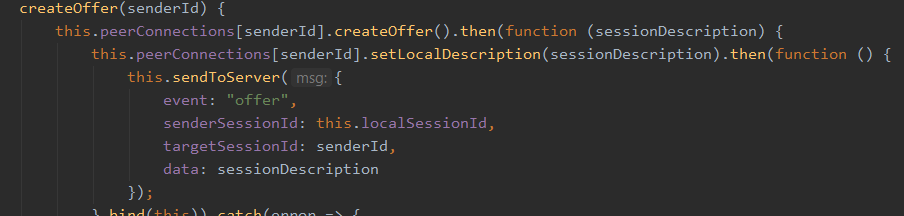
\includegraphics[width=1\textwidth]{resources/createOfferBeispiel.png}
    \caption{Codeausschnitt CreateOffer()-Methode}
    \label{fig:createOffer}
\end{figure}

Bei jeder Nachricht während des Signaling-Prozesses muss immer die Session-ID des Senders und des Empfängers angegeben werden, damit
der Server die Weiterleitung an den entsprechenden Client abwickeln kann, und der Empfänger die Nachricht dem entsprechenden
RTCPeerConnection-Objekt des Senders zuordnen kann.
Zusätzlich muss immer ein Nachrichten-Typ übermittelt werden, damit der Empfänger weiß wie er das SDP der Nachricht verarbeiten muss und wie er antworten muss.
Dafür muss im clientseitigen onMessage Event des WebSockets eine Differenzierung, je nach empfangenen Nachrichten Typ erfolgen.
\newpage

\subsection{UI}
\label{subsec:DatenaustauschUI}
Nachdem sich beide \textit{peers} auf einen ICE-Kandidaten geeinigt haben, und somit die Medien-Daten austauschen können,
wird das \textit{onTrack}-Event der \textit{peers} ausgelöst\footnote{Die addTrack()-Methode löst das onTrack-Event des RTCPeerConnection-Objektes
auf der Remote Seite aus, nicht bei dem lokalen RTCPeerConnection-Objekt}.
Die MediaStreamTrack-Objekte werden den RTCPeerConnection-Objekten bereits nach deren Initialisierung zugewiesen, sofern dann schon ein MediaStream-Objekt
vorhanden ist.

\begin{figure}[h]
%figure full paperwidth and trim the left and right empty space from it
    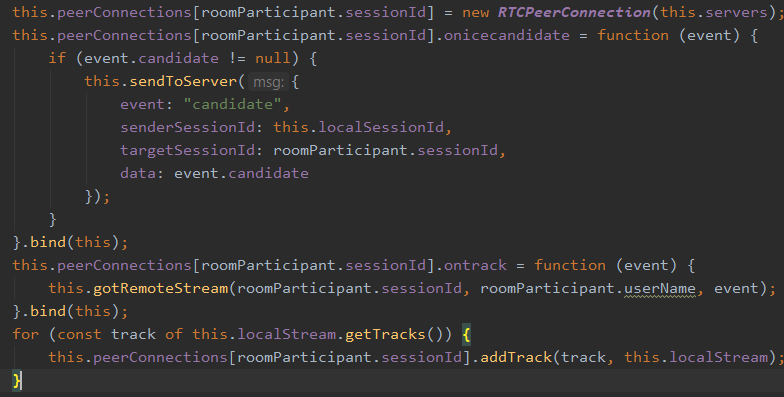
\includegraphics[width=1\textwidth]{resources/mediaStreamTracks.png}
    \caption{Codeausschnitt Datenaustausch}
    \label{fig:Datenaustausch}
\end{figure}

Im Event-Handler des \textit{onTrack }-Events kann nun auf den übertragenen MediaStream, und dessen Tracks, des anderen \textit{peers} zugegriffen werden.
Für die Oberfläche dieser Anwendung wird im Event-Handler eine Funktion aufgerufen in der für jeden neuen MediaStream ein
HTMLVideo-Element erstellt, und mit der \textit{append()}-Methode in den DOM eingefügt, wird.
Da das HTMLVideo-Element das HTMLMedia-Element-Interface implementiert kann als Wiedergabe-Quelle ein
MediaStream-Objekt gesetzt werden\parencite{WebDocsSrcObject}.

\newpage

\subsection{WebComponent}
\label{subsec:webcomponent}
Um eine möglichst hohe Wiederverwendbarkeit und leichte Anpassung für andere Projekte zu ermöglichen,
wurde die clientseitige Logik als sogenannte WebComponent gekapselt.
Dabei handelt es sich um ein benutzerdefiniertes HTML-Element, welches mit einer Javascript-Klasse verknüpft ist und
die dort definierte Funktionalität über die zu implementierende Methode \textit{connectedCallback()} ausführt sobald es vom DOM
mit dem Dokument verbunden wird.
Die Verknüpfung des <video-conference>-Elementes mit der VideoConference-Klasse wird durch die CustomElementRegistry.define()-Methode registriert.
Die VideoConference-Klasse muss zudem von der HTMLElement-Klasse erben.
Wenn die Logik nun in einem anderen Projekt für Videokonferenzen verwendet wird, kann
der Endpunkt des Signaling-Servers über die HTML-Attribute \textit{socketHostname} und \textit{socketPathname} modifiziert werden, ohne den Javascript-Code
anpassen zu müssen.
Die Existenz und der Wert dieser Attribute wird in der connectedCallback()-Methode abgefragt.
\begin{figure}[h]
    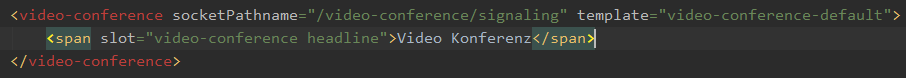
\includegraphics[width=1\textwidth]{resources/customElement.png}
    \caption{Codeausschnitt Custom <video-conference>-Element}
    \label{fig:CustomElement}
\end{figure}

Um zudem die Element-Struktur, das Styling und das Verhalten vom restlichen Code der Anwendung abzugrenzen wird
die Shadow DOM API genutzt.
Dabei handelt es sich um einen versteckten separaten DOM der an ein Element angehangen wird und nicht
von den Styles und definierten Verhalten des Standard-DOMs betroffen \parencite{WebDocsShadowDOM}.
